\documentclass[a4paper]{article}

\usepackage[style=numeric]{biblatex}
\usepackage{graphicx}
\usepackage{enumitem}
\usepackage{geometry}
\usepackage{sectsty}
\usepackage{indentfirst}

\setlist{
  listparindent=\parindent,
  parsep=0pt,
}

\sectionfont{\centering}
\addbibresource{citation.bib}
\graphicspath{{./images/}}
\geometry{a4paper, top=4.0cm, bottom=3.0cm,
          left=4.0cm, includehead, includefoot}
\renewcommand\contentsname{Daftar Pustaka}

\begin{document}
\linespread{1.5}

\title{SSD (Single Shot Detector) and DeepForest Algorithm Comparison}
\author{Aldih Suhandi, Chandra Wijaya, Ibrahim Seto Aditama}

\maketitle

\newpage

\addcontentsline{toc}{section}{\protect\numberline{}Daftar Pustaka}
\tableofcontents
\newpage

\section*{Tinjauan Pustaka}
\addcontentsline{toc}{section}{\protect\numberline{}Tinjuan Pustaka}
\begin{enumerate}

    \item \textbf{\textit{SSD with Feature Selective Anchor-Free Module}}

    SSD menggunakan \textit{anchor mechanism}, mekanism sama yang digunakan didalam \textit{Faster R-CNN} untuk menemukan target yang akan diprediksi. SSD akan melakukan extraksi dibeberapa \textit{anchor points} yang berbeda dan akan juga memprediksi \textit{anchor boxes} dengan rasio tinggi dan lebar yang berbeda di \textit{anchor points} yang sama \autocite{19532655}. Design ini mengandalkan \textit{anchor point} yang didefinisikan oleh manusia dan memiliki overlap yang cukup dengan \textit{ground truth} \autocite{FCOS-1}, oleh karena ini design memiliki beberapa limitasi seperti:
    \begin{enumerate}
        \item pemilihan feature yang dilakukan secara heuristic
        \item ketergantungan dengan \textit{anchor sampling}
    \end{enumerate}

    Saat melakukan \textit{training}, setiap instance selalu mencoba mencocokan item dengan \textit{anchor box} yang paling sesuai bedasarkan \textbf{IoU} atau \textit{Intersection over Union}. Hal ini menyebabkan pengklasifikasian item bedasarkan \textit{anchor box} yang sudah didefinisikan SSD atau algoritma lain yang menggunakan approach ini mungkin tidak optimal\autocite{Zhu_2019_CVPR}.


    \begin{figure}[h]
        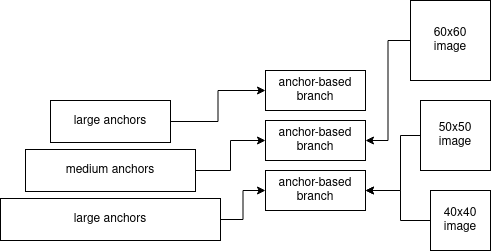
\includegraphics[width=8cm]{general_architectur_anchor_based.png}
        \centering

        \caption{feature level yang dipilih di \textit{anchor based} mungkin tidak optimal \autocite{Zhu_2019_CVPR}.}
    \end{figure}

    
    Karena dua kelemahan ini, para peneliti mulai berarah ke detector yang tidak menggunakan \textit{Anchor} ini, seperti \textbf{FPN} dan \textbf{\textit{Focal Loss}} atau bisa disebut juga \textbf{\textit{Anchor-Free Detector}}\autocite{Zhang_2020_CVPR}, detector type ini bisa menemukan obyek secara langsung tanpa \textit{preset anchor} dengan dua cara berbeda:

    \begin{itemize}
        \item \textbf{\textit{Key Point Base Method}}

            metode ini pertama mencoba untuk mencari beberapa titik yang sudah didefinisikan sebelumnya atau titik yang dipelajari, untuk membuat sebuah kotak pembatas yang mungkin ada sebuah obyek yang bisa diklasifikasikan\autocite{DBLP:journals/corr/abs-1904-03797}.

        \item \textbf{\textit{Center Base Method}}

            metode ini menganggap pusat (misalnya, titik pusat atau bagian) dari obyek sebagai latar depan untuk mendefinisikan \textit{positive} dan memprediksi jarak dari sebuah \textit{positive} ke empat sisi \textit{bounding box} yang nanti akan digunakan untuk proses deteksi\autocite{Zhang_2020_CVPR}.


            Salah satu algoritma yang menggunakan konsep ini adalah \textit{Point Linking Network (\textbf{PLN})}, untuk memprediksi sebuah \textit{bounding box} dilakukan dalam beberapa tahap, yaitu:

            \begin{itemize}
                \item memprediksi lokasi dari empat titik sudut dan titik tengah dari suatu \textit{bounding box};
                \item setelah itu ditiap lokasi titik sudut, algorithma inni memprediksi sebeapar besar kemungkinan tiap lokasi pixel untuk menjadi titik tengah sebuah objek;
                \item hal yang sama pun dilakukan dititik tengah \textit{bounding box}, tapi untuk memprediksi seberapa besar kemugnkinan tiap pixel itu berada di kiri atas, pojok kanan atas, kiri bawah, atau pojok kanan bawah;
                \item setelah selesai, algoritma ini akan menggabungkan prediksi dari tiap sudut dan titik tengah untuk membuat suatu \textit{boundig box}\autocite{DBLP:journals/corr/abs-1808-01244}.
            \end{itemize}

    \end{itemize}


    Dari \textit{paper} yang mengusulkan menggunakan \textbf{FSAF} atau \textit{Feature Selective Anchor Free}, solusi mereka adalah membiarkan tiap instance memilih feature level yang terbaik untuk mengoptimasi \textit{network item} yang dibuat, dengan mengganti \textit{anchor box} yang biasanya mebatasi pemilihan feature disebuah module menjadi instance dengan \textit{anchor-free manner} untuk mempelajari parameter - parameter yang dibutuhkan untuk melakukan proses klasifikasi dan regresi\autocite{Zhu_2019_CVPR}.

    \begin{figure}[h]
        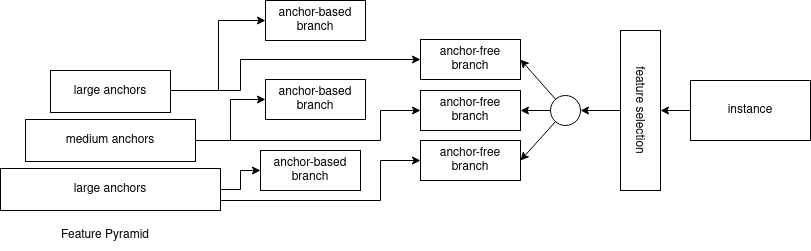
\includegraphics[width=8cm]{basic_overview_FSAF.png}
        \centering
    
        \caption{basic overview dari module \textit{anchor free} yang dipasang ke detection method yang menggunakan \textit{anchor}\autocite{Zhu_2019_CVPR}.}
    \end{figure}
\end{enumerate}

\newpage
\section*{Metode Penelitian}
\addcontentsline{toc}{section}{\protect\numberline{}Metode Penelitian}

\subsection*{Jenis Penelitian}
\addcontentsline{toc}{subsection}{\protect\numberline{}Jenis Penelitian}
Jenis penelitian yang dilakukan adalah penelitian kuantitatif atau penelitian sistematis yang memakai data atau angka - angka yang ditambahkan penekanan terhadap pengukuran hasil yang obyektif disertai analisis statistik\autocite{pengajar-1} dan penelitian ini juga bersifat komparatif atau penelitian yang dilakukan dengan cara membandingkan persamaan atau perbedaan dari dua atau lebih atribut yang dimiliki oleh sesuatu\autocite{penerbitdeepublish-1}.

\subsection*{Fokus Penelitian}
\addcontentsline{toc}{subsection}{\protect\numberline{}Fokus Penelitian}
Kajian penelitian ini difokuskan pada perbandingan dari dua algorithma pendekteksi yaitu \textbf{SSD \textit{(Single Shot Detection)}} dan \textbf{\textit{DeepForest Algorithm}}, hal yang akan penulis observasi adalah bagaimana dua algoritma ini berfungsi dan seberapa bagus performa mereka dalam berbagai macam situasi.

Variabel yang penulis akan perhatikan adalah \textit{time cost} atau seberapa lama waktu yang dibutuhkan oleh algoritma tersebut untuk melakukan fungsinya (waktu \textit{training} dan waktu \textit{prediction}) dan akurasi, seberapa akurat sebuah algorithma untuk mendeksi suatu obyek, seperti seberapa akurat \textit{bounding box} yang dibuat atau persentase obyek yang terdeteksi oleh algoritma tersebut dibanding dengan berapa banyak obyek yang ada disuatu gambar atau video.


\subsection*{Teknik Pengumpulan Data}
\addcontentsline{toc}{subsection}{\protect\numberline{}Teknik Pengumpulan Data}
Teknik pengumpulan data merupakan teknik atau metode yang digunakan untuk mendapatkan data yang akan diteliti. Artinya, teknik pengupulan data memperlukan langkah yang strategis dan juga sistematis untuk mendapatkan data yang valid dan juga sesuai dengan kenyataannya\autocite{penerbitdeepublish-2}.

Dalam hal pengumpulan data ini, penulis langsung melakukan percobaan pada obyek penelitian untuk mendapatkan data yang valid dan bisa direproduksi untuk mevalidasi data yang dihasilkan. Teknik yang digunakan penulis adalah teknik observasi atau pengamatan, dengan cara mengobservasi \textit{output} atau hasil apa yang diberikan saat suatu algoritma pendekteksi diberikan \textit{input} tertentu.

\newpage
\addcontentsline{toc}{section}{\protect\numberline{}Referensi}
\printbibliography[title=Referensi]

\end{document}